\documentclass{HZNUMCM}
\usepackage{graphicx}
\usepackage{hyperref}
\usepackage{subcaption}
\usepackage{float}
\usepackage{svg}
\usepackage{mathrsfs}

\definecolor{customcolor}{HTML}{429938}

\setControlNumber{2511940}
\setContestType{MCM}
\setProblemLetter{E}
\setPaperTitle{Our Article}

%summary
\setSummary{ sumary sumary sumary sumary sumary sumary sumary sumary sumary sumary sumary sumary sumary sumary sumary sumary sumary sumary sumary sumary sumary sumary sumary sumary sumary sumary sumary sumary sumary sumary sumary sumary sumary sumary sumary sumary sumary sumary sumary sumary sumary sumary sumary sumary sumary sumary sumary sumary sumary sumary sumary sumary sumary sumary sumary sumary sumary sumary sumary sumary sumary sumary sumary sumary sumary sumary sumary sumary sumary sumary sumary sumary sumary sumary sumary sumary sumary sumary sumary sumary sumary sumary sumary sumary sumary sumary sumary sumary sumary sumary sumary sumary sumary sumary sumary sumary sumary sumary sumary sumary sumary sumary sumary sumary sumary sumary sumary sumary sumary sumary sumary sumary sumary sumary sumary sumary sumary sumary sumary sumary sumary sumary sumary sumary sumary sumary sumary sumary sumary sumary sumary sumary sumary sumary sumary sumary sumary sumary sumary sumary sumary sumary sumary sumary sumary sumary sumary sumary sumary sumary sumary sumary sumary sumary sumary sumary sumary sumary sumary sumary sumary sumary sumary sumary sumary sumary sumary sumary sumary sumary sumary sumary sumary sumary sumary sumary sumary sumary sumary sumary sumary sumary sumary sumary sumary sumary sumary sumary sumary sumary sumary sumary sumary sumary sumary sumary sumary sumary sumary sumary sumary sumary sumary sumary sumary sumary sumary sumary sumary sumary sumary sumary sumary sumary sumary sumary sumary sumary sumary sumary sumary sumary sumary sumary sumary sumary sumary sumary sumary sumary sumary sumary sumary sumary sumary sumary sumary sumary sumary sumary sumary sumary sumary sumary sumary sumary sumary sumary sumary sumary sumary sumary sumary sumary sumary sumary sumary sumary sumary sumary sumary sumary sumary sumary sumary sumary sumary sumary sumary sumary sumary sumary sumary sumary sumary sumary sumary sumary sumary sumary sumary sumary sumary sumary sumary sumary sumary sumary sumary sumary sumary sumary sumary sumary sumary sumary sumary sumary sumary sumary sumary sumary sumary sumary sumary sumary sumary sumary sumary sumary sumary sumary sumary sumary sumary sumary sumary sumary sumary}

%begin
\begin{document}
\showSummarySheet
\showContents

  \section{Introduction}
    \subsection{Background}
    In the past few decades, with the rapid population growth, 
    food supply has become one of the most pressing global issues. 
    Under the conditions where scientific and technological advancements have not been fully adopted, 
    the existing arable land area is insufficient to meet the food demand. 
    As a result, many regions have resorted to deforestation for land conversion, 
    as shown in \figurename~\ref{fig:deforestation1}. \figurename~\ref{fig:deforestation2} illustrates that when the forest ecosystem is artificially disrupted, 
    its complex spatial structure is destroyed.
    \begin{figure}[H]
      \centering
        \begin{minipage}[b]{0.45\linewidth}
            \centering
            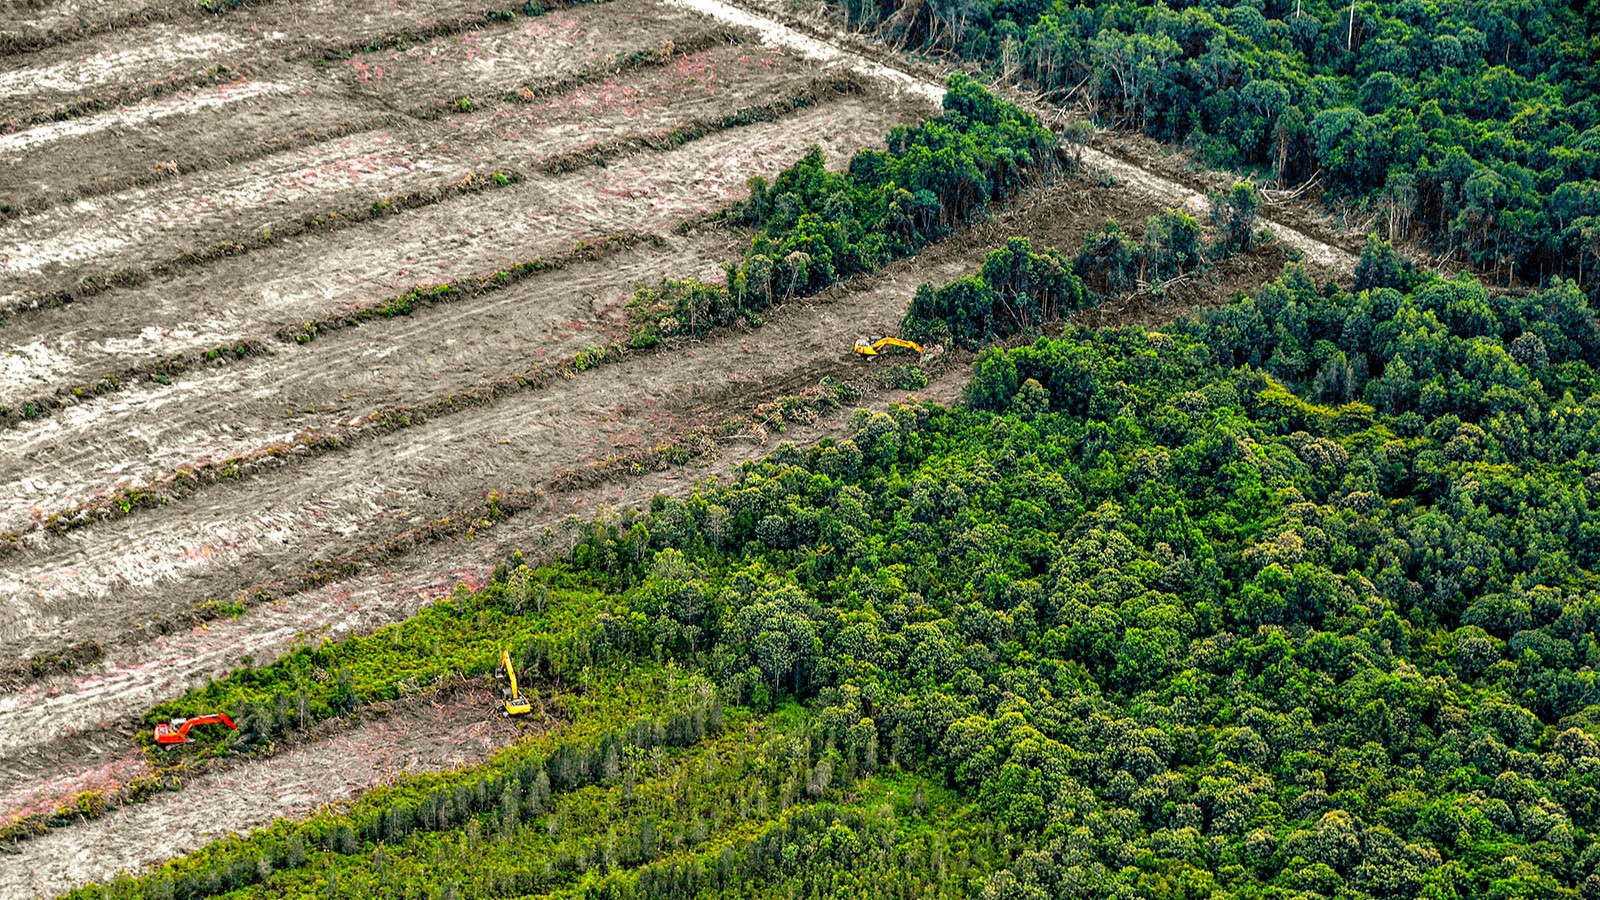
\includegraphics[height=4cm, keepaspectratio]{images/deforestation1.jpg} % 替换为你的第一张图片路径
            \caption{Deforestation for Farming}
            \label{fig:deforestation1}
        \end{minipage}
      \hspace{0.05\linewidth}
        \begin{minipage}[b]{0.45\linewidth}
            \centering
            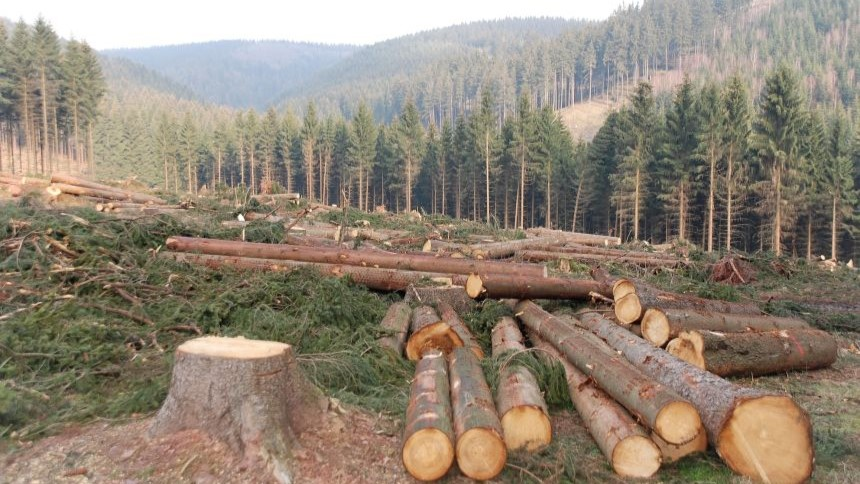
\includegraphics[height=4cm, keepaspectratio]{images/deforestation2.jpg} % 替换为你的第二张图片路径
            \caption{Deforested Forest}
            \label{fig:deforestation2}
        \end{minipage}
      \end{figure}
    Therefore, the converted forest area must undergo a long process of ecological reconstruction. 
    However, due to the influence of human activities during this process, 
    the post-clearing forest ecosystem can no longer return to its original state, 
    but instead continuously undergoes succession into a stable agricultural ecosystem. 
    To achieve both economic and ecological benefits and fulfill sustainable development goals, 
    it is necessary to examine the ecological succession from converted forest to agricultural ecosystems and explore how green agriculture can bring dual benefits in terms of economic and ecological indicators.
      
    \subsection{Problem Analysis}
      The basic requirements of the project are to establish a model that reflects the ecological succession process from a converted forest area to a mature agricultural ecosystem over time. 
      The model should incorporate both natural processes and human agricultural activities. 
      Specifically, the requirements are as follows:
      \begin{itemize}
        \item \textbf{Develop an ecological model} for the converted forest area, particularly:
          \begin{itemize}
            \item \textbf{Food web construction}: The model should include at least producers (e.g., plants) and consumers (e.g., herbivores and predators) and their interactions.
            \item \textbf{Consideration of agricultural cycles and seasonality}: The impact of seasonal and cyclical agricultural activities should be taken into account.
            \item \textbf{Impact of chemicals}: The model should account for the effects of chemicals such as herbicides and pesticides on plants, insects, bats, birds, and the stability of the ecosystem.
          \end{itemize}
        \item \textbf{Reemergence of species during ecosystem maturation}: As the ecosystem matures, the model should consider the reemergence of two species and their impact on the ecosystem.
        \item \textbf{Impact of removing chemicals}: After the ecosystem matures, humans will attempt to remove chemicals. The model should assess the stability of the ecosystem after herbicides are removed, with the effects reflected through producers and consumers.
        \item \textbf{Introduction of bats into the food web}: The model should examine how bats, as insectivores and pollinators, interact with plants, insects, and predators, and how their inclusion influences the stability of the ecosystem. Additionally, the model should identify another species that could benefit the ecosystem and compare the effects of different species.
        \item \textbf{Analysis of the impact of organic farming}: The model should assess the impact of adopting organic farming practices, considering various scenarios and components. The evaluation should include the effects on the overall ecosystem and individual elements, such as pest control, crop health, plant reproduction, biodiversity, long-term sustainability, and cost-effectiveness. The model should analyze the impact of organic practices on pest management, soil health, and biodiversity, while weighing the economic costs and benefits. A comprehensive ecological and economic trade-off analysis should be provided to assess the feasibility of organic farming.
      \end{itemize}

    \subsection{Our Work}
    \begin{itemize}
      \item 1
      \item 2
      \item 3
    \end{itemize}

  \section{Assumptions and Notations}
    \subsection{Assumptions and Explanations}
      \begin{itemize}
        \item \textbf{Accurate Data Assumption}: The model assumes that the data used are accurate.\\
        \textbf{Explanation}: The data used in the model are sourced from official databases, and we believe the data to be accurate and reliable.
        
        \item \textbf{Geographic Applicability Assumption}: The model assumes that the applicable region is Southeast Asia,
         where two crops of rice are planted each year in the farmland.\\
        \textbf{Explanation}: The climate of Southeast Asia is rather simple, 
        with only two seasons-rainy and dry. Additionally, as is shown in \figurename~\ref{fig:Temperature},
        the temperature variation within a year is minimal,which has a trivial effect on the ecosystem.
        Consequently,temperature can be considered as a constant.
        Due to such weather pattern,it aligns with the planting patterns commonly observed in Southeast Asia to plant two crops of rice each year,
         and the simplicity of crop types makes the model easier to establish.
        
        \begin{figure}[H]
          \centering
          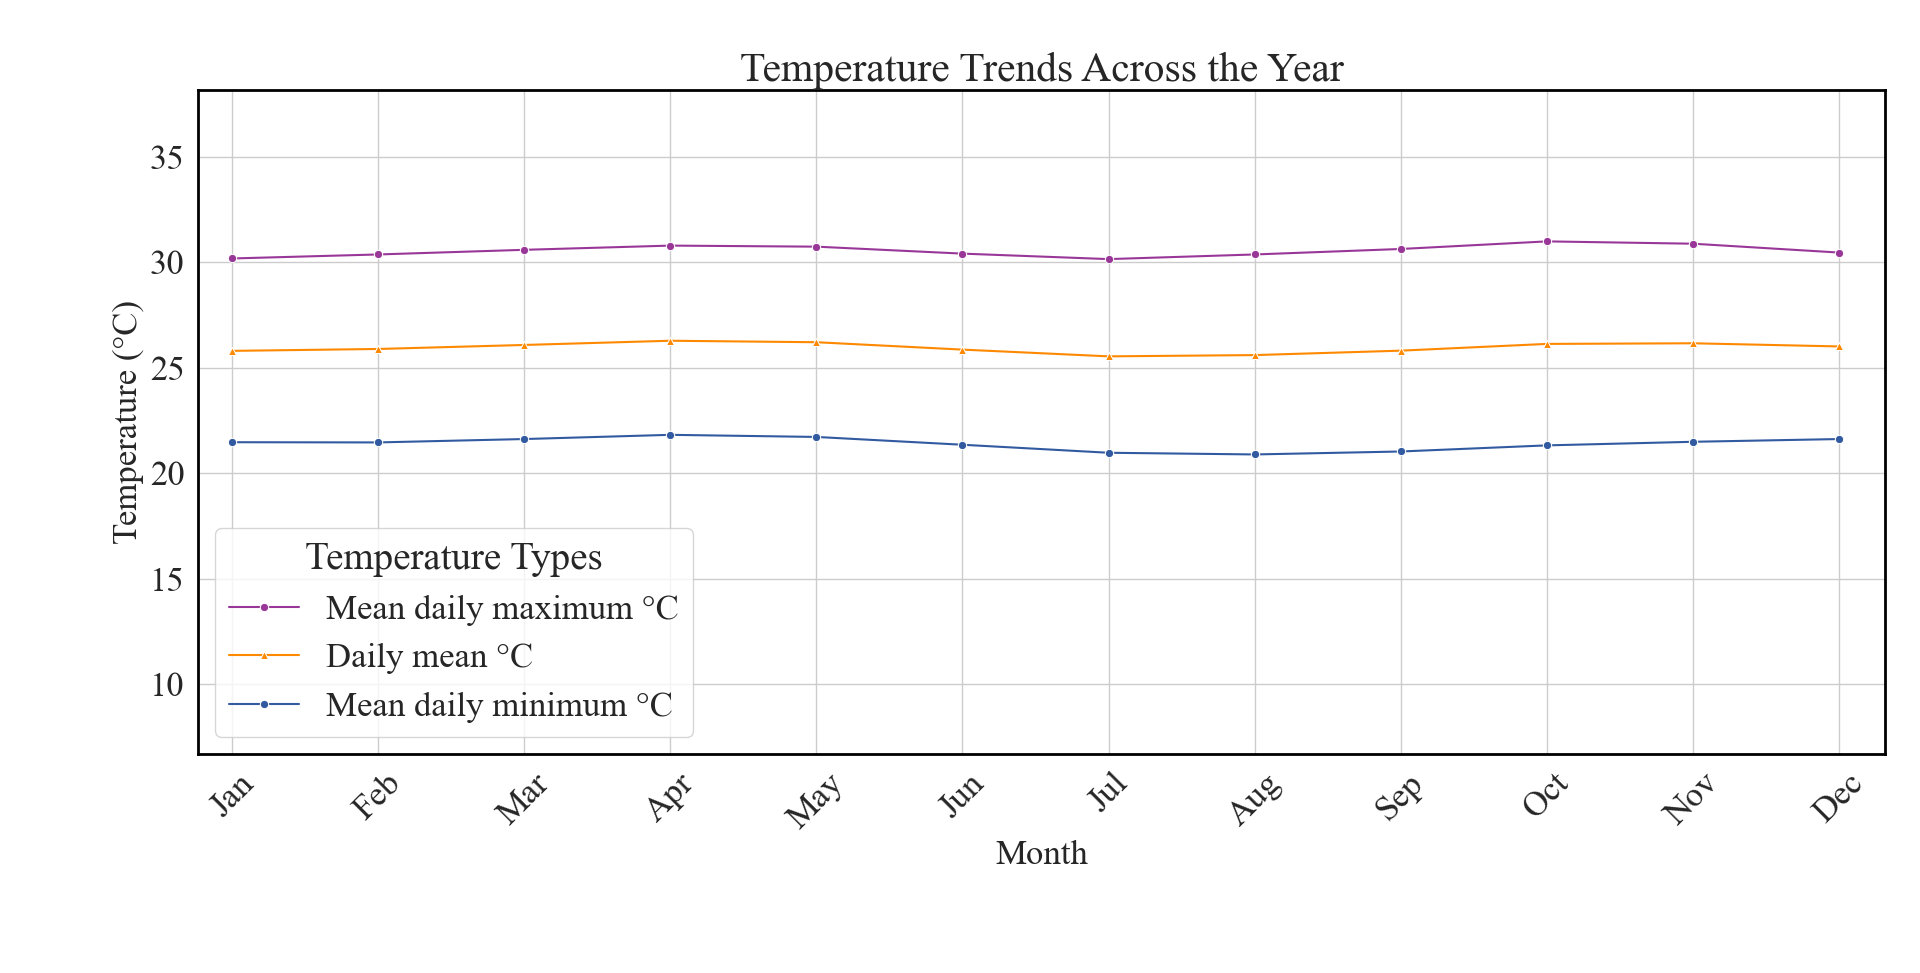
\includegraphics[width=\linewidth]{images/AverTemper.png}
          \caption{Mean Temperature from 1991 to 2020 in Southeast Asia}
          \label{fig:Temperature}
        \end{figure}

        \item \textbf{Stable Trait Assumption}: The model assumes that the traits of all organisms remain stable.\\
        \textbf{Explanation}:Since the time span considered in the model is much shorter than the time required for evolutionary changes or mutations to occur,
         the traits of organisms are assumed to remain stable. This assumption also helps simplify the model.
        
        \item \textbf{Stable Lighting Conditions Assumption}: The model assumes that the region under study experiences stable lighting conditions throughout the four seasons.\\
        \textbf{Explanation}: Since the model focuses on tropical regions, the variation in daylight duration across different months within a year is minimal,
         thus the lighting conditions are treated as constant in the model.
        
        \item \textbf{Stable Growth Environment Assumption}: The model assumes that no natural disasters,
         which could significantly impact the agricultural ecosystem, will occur during the time frame considered.\\
        \textbf{Explanation}: Natural disasters are considered low-probability events in agricultural activities.
         To ensure the generalizability of the model, natural disasters should not be considered.
      \end{itemize}

        \subsection{Notations}
      % table
      \begin{table}[H]
        \centering
        \caption{Notations}
        \begin{tabular}{cc}
          \toprule
          \rowcolor{customcolor!40} % 设置背景颜色
          Symbols & Description\\
          \midrule
          $\mathbf{X}$ & Vector $[N_{wd},N_{crp},N_{pst},N_{ins},...,C_{hc},C_{pc}]^T$ to describe the system,etc. \\
          $wd$ & Subscription for weeds \\
          $crp$ & Subscription for crops \\
          $pst$ & Subscription for pest(who consumes crops) \\
          $ins$ & Subscription for other insects(who consume weeds) \\
          $bd$ & Subscription for small birds(herbivorous) \\
          $Bd$ & Subscription for huge birds(carnivorous) \\
          $bt$ & Subscription for bats \\
          $snk$ & Subscription for snake \\
          $frg$ & Subscription for frog \\
          $HC$ & Subscription for herbicide \\
          $PC$ & Subscription for pesticide \\
          $C_i$ & Concentration of certain chemical \\
          $N_i$ & Numbers of certain species \\
          $W_i$ & Biomass of certain species \\
          $w_i$ & Average mass of individuals of certain individuals \\
          $r_i$ & Natural growth gate of certain population\\
          $\mathscr{K}_i$ & Carrying capacity of certain population\\
          $\alpha$ & The effect of chemical concentration on growth rate\\
          $\beta_{i \rightarrow j}$ & Interspecific competition factor\\
          $\gamma$ & Activity of decomposer\\
          $A_i,B_i$ & Effect of the predator-prey relationship on population $i$ (specified coefficient).\\
          $N,P,K$ & Chemical elements\\
          \bottomrule
        \end{tabular}
        \label{tab:Notations}
      \end{table}

  \section{Models}
    \subsection{LVLG(Lokta-Volterra and Leslie-Gower) Model}
      The components of an ecosystem are complex and interdependent. 
      However, in a converted forest area, the ecosystem could be rather simple.
      Set February-when rice has just been planted-as the start time.
      Around the start time, in the simplest case, when climate, soil, and other conditions are favorable, 
      only biological factors should be considered.
      If the population sizes of producers and primary consumers are used to describe the entire system, 
      the Lotka-Volterra Model\cite{wangersky1978lotka} and Leslie-Gower Model\cite{GUO20142850} can be applied as follows:
      \begin{equation}
        \begin{aligned}
          \frac{\mathrm{d}W_{crp}}{\mathrm{d}t}&=r_{crp}W_{crp}\left( 1-\frac{W_{crp}+\beta _{w\rightarrow c}W_{wd}}{\mathscr{K} _{crp}} \right) -\frac{A_{crp}W_{crp}W_{ins}}{1+B_{crp}W_{crp}}\\
          \frac{\mathrm{d}W_{wd}}{\mathrm{d}t}&=r_{wd}W_{wd}\left( 1-\frac{W_{wd}+\beta _{c\rightarrow w}W_{crp}}{\mathscr{K} _{wd}} \right) -\frac{A_{wd}W_{wd}W_{ins}}{1+B_{wd}W_{wd}}\\
          \frac{\mathrm{d}W_{ins}}{\mathrm{d}t}&=r_{ins}W_{ins}\left[ 1-\frac{D_{ins}W_{ins}}{1+E_{ins}\left( 0.6W_{crp}+0.4W_{wd} \right)} \right] -\frac{A_{ins}W_{ins}W_{bd}}{1+B_{ins}W_{ins}}\\
          \frac{\mathrm{d}W_{bd}}{\mathrm{d}t}&=r_{bd}W_{bd}\left( 1-\frac{D_{bd}W_{bd}}{1+E_{bd}W_{ins}} \right)\\
        \end{aligned} 
      \end{equation}
      
      The notations can be seen in Table \ref{tab:Notations},ans the following points provide explanations of the model.

      First, biomass is chosen over population density because rice, 
      as the primary producer in the agricultural ecosystem, 
      has its population density artificially determined (i.e., it does not reproduce). 
      Only the changes in its total biomass can reflect the developmental trend of the rice population.
      
      Second, regarding interspecific competition, since the agricultural ecosystem is relatively simple at this stage, 
      for the sake of model simplification, only interspecific competition between rice and weeds is considered. 
      The model presented later similarly assumes this.

      Next, for the purpose of further simplifying the model, some parameters are combined. 
      For example, the predation rate is incorporated into the predation coefficient of the prey species, denoted as \(A\).
      
      Finally, since consumers are in a natural reproductive state with a relatively fixed age structure, the average individual biomass can be assumed to be constant. Therefore, biomass is directly proportional to the number of individuals in the population, and this assumption applies similarly in the following sections.
      
      It should be noted that at the start time, all the variations and coefficients mentioned above are positive real numbers.
      \subsection{NGLG(Natrual Growth Leslie-Gower) Model}
      \subsubsection{NGLG Model}
      \begin{figure}[H]
        \centering
          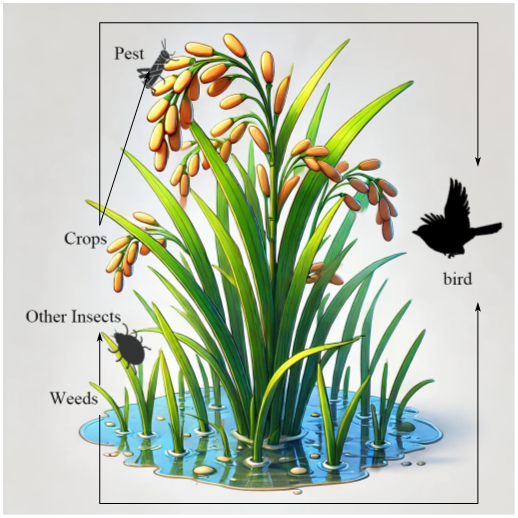
\includegraphics[width=0.5\linewidth]{images/init_crop_field.png} 
          \caption{Crop Field for LG Model}
          \label{fig:LG_Field}
      \end{figure}
      \begin{figure}[H]
          \centering
          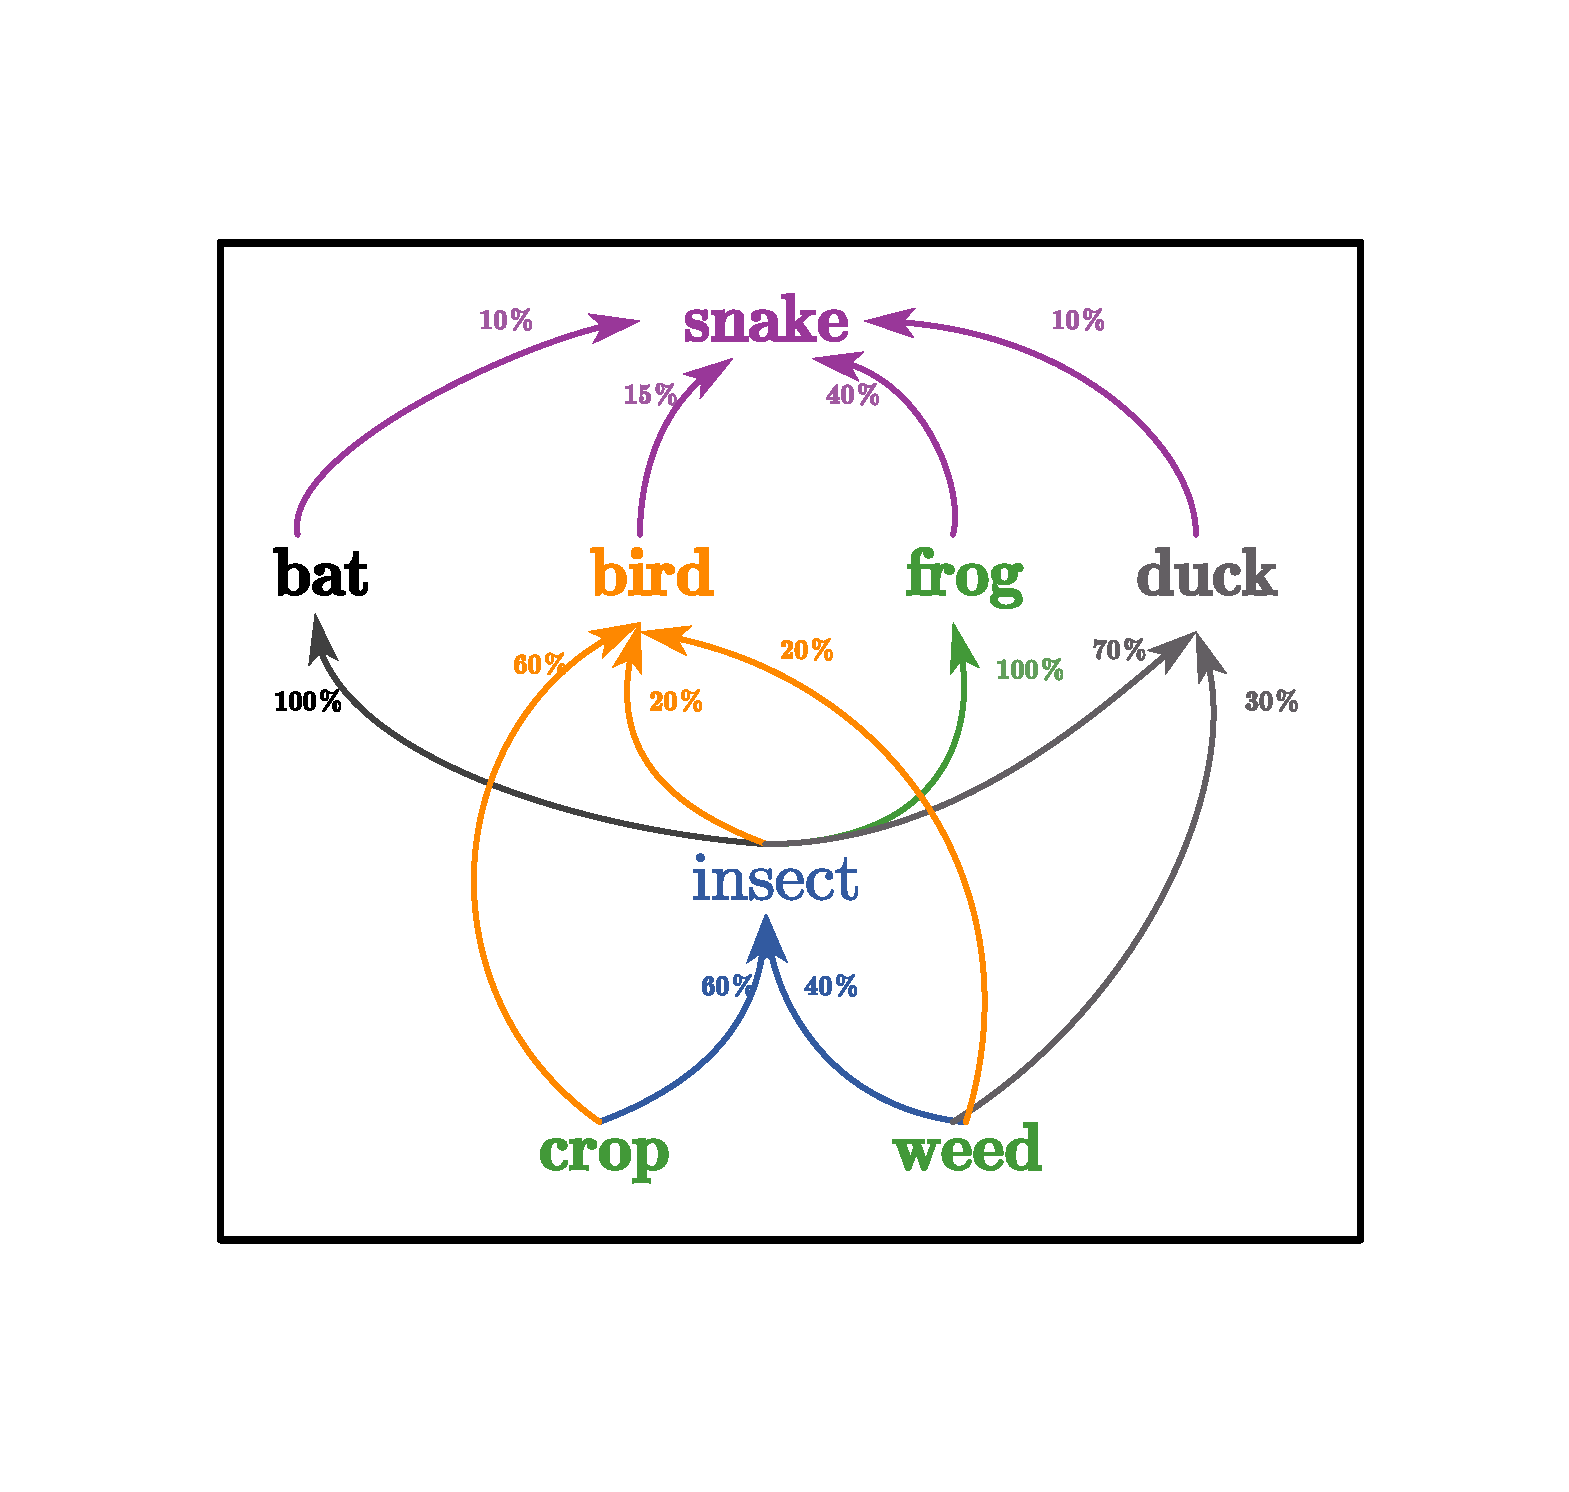
\includegraphics[width=0.8\linewidth]{images/food_web.pdf}
          \caption{Food web for NGLG Model}
          \label{fig:NGLG_FoodWeb}
      \end{figure}
        
  \section{Application of the Models}

  \section{Sensitivity Analysis}

  \section{Evaluation of the Model}
    \subsection{Strengths}
    \subsection{Weaknesses}

  \section{Conclusion}

  %%citation
  % as \figurename~\ref{fig:image1} shows,this is a picture.
  % ...\cite{example1}
  % 123123123\cite{rosenow1983drought}

  \addcontentsline{toc}{section}{References}
  \bibliographystyle{unsrt}%{brief}%{alpha}%{unsrt}
  \bibliography{article_file}

\end{document}